\documentclass[a4paper,12pt]{article}

\usepackage[utf8]{inputenc}
\usepackage{graphicx}
\usepackage[dvipsnames]{xcolor}

%\usepackage[defaultmono]{droidmono}
\usepackage{wrapfig}

\usepackage{amsmath,amssymb,amsthm,textcomp}
\usepackage{enumerate}
\usepackage{multicol}
\usepackage{tikz}
\usepackage{listings}
%\usepackage{pst-plot}
\usepackage{geometry}
\usepackage{sidecap}
\geometry{total={210mm,297mm},
left=25mm,right=25mm,%
bindingoffset=0mm, top=20mm,bottom=20mm}


\linespread{1.3}

\newcommand{\linia}{\rule{\linewidth}{0.5pt}}

%\savedata{\data}[{{0,0},{1,1},{2,11},{3,6},{4,6},{5,3},{6,2},{7,0},{8,0},{9,1},{10,1},{11,0},{12,1},{13,0},{14,0},{15,0},{16,1},{17,1}}]

%\renewcommand\lstlistingname{Code}

\definecolor{backcolour}{rgb}{0.95,0.95,0.95}

\lstset{%
    backgroundcolor=\color{backcolour},
    basicstyle=\ttfamily\scriptsize,
    breaklines=true,
    captionpos=t,
    numbers=left,
    numberstyle=\tiny,
    numbersep=5pt,
    frame=tb,
    commentstyle=\color{PineGreen},
    keywordstyle=\color{RoyalBlue}
}

% custom theorems if needed
% my own titles
\makeatletter
\renewcommand{\maketitle} {%
\begin{center}
\vspace{2ex}
{\huge \textsc{\@title}}
\vspace{1ex}
\\
\linia\\
\@author \hfill \@date
\vspace{4ex}
\end{center}
}
\makeatother
%%%

% custom footers and headers
\usepackage{fancyhdr}
\pagestyle{fancy}
\lhead{}
\chead{}
\rhead{}
\lfoot{Complex Network \textbar \ Assignment 2}
\cfoot{}
\rfoot{15M54097 - Page \thepage}
\renewcommand{\headrulewidth}{0pt}
\renewcommand{\footrulewidth}{0pt}
%

% code listing settings
%%%----------%%%----------%%%----------%%%----------%%%

\newcommand*{\quoteTitle}[1]{{#1}\ignorespaces}%
\newenvironment{Quote}[1]{
    \medskip\par\noindent\quoteTitle{#1}
    \par\noindent
    \begin{quote}
    }{
    \end{quote}
    \par\noindent\ignorespacesafterend
}

\newtheorem{theorem}{Theorem}

\begin{document}
\bibliographystyle{acm}
\title{Complex Network - Assignment 2}

\author{NGUYEN T. Hoang - SID: 15M54097}

\date{Fall 2015, W833 Mon. Period 5-6 \\ \hfill Due date: 2016/02/01}

\maketitle

\vspace{4em}
\section*{Problem}
\noindent
Given a network as in Figure~\ref{fig:net}. Complete these following tasks:
\begin{enumerate}
    \item Compute eigenvector centrality and betweenness centrality of each vertex in the given network.
    \item Find eigenvectors of matrices, construct the Laplacian and the modularity matrix for this small network:
    \begin{enumerate}
        \item Find the eigenvector of the Laplacian corresponding to the second smallest eigenvalue and hence perform a spectral bisection of the network into two equally sized parts.
        \item Find the eigenvector of the modularity matrix corresponding to the largest eigenvalue and hence divide the network into two communitites.
    \end{enumerate}
    \item Explain quantitatively why ``\emph{your friends have more friends than you do}'' in the configuration model.
    \item Write examples of parameters $\beta$ and $\gamma$ of SIR model when:
    \begin{enumerate}
        \item There is an epidemic.
        \item There is no epidemic.
    \end{enumerate}
\end{enumerate}
\pagebreak
\section*{Answer}

\noindent
In this assignment, I will use SNAP.PY, a network analysis developed by Stanford University, as a computational tool. All illustrations (figures, graphs \ldots) are drawn using D3 Javascript Framework.

\paragraph{Question 1:} Compute eigenvector centrality and betweenness centrality of each vertex.

\begin{figure}[h]
    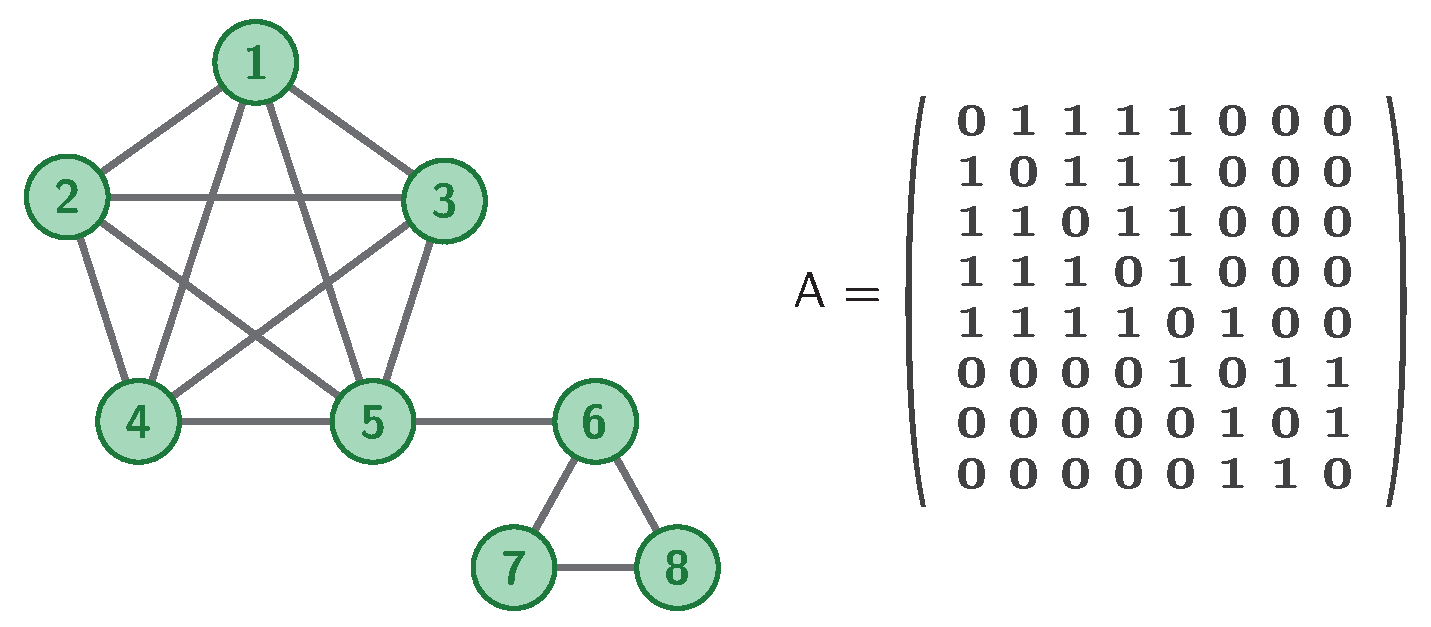
\includegraphics[width=\textwidth]{cn_a2_net}
    \caption{Simple network and its corresponding adjacency matrix.}
    \label{fig:net}
\end{figure}

\noindent
\emph{Eigenvector centrality} is given by the formula:
$$ x_i^{(t)}= \Sigma_{j \neq i} A_{ij} \times x_i^{(t)} $$
Rewrite in final matrix form:
$$ A\boldsymbol{x} = k_1\boldsymbol{x} $$
where $\boldsymbol{x}$ is a vector storing score of all nodes, and $k_1$ is the largest eigenvalue of the adjacency matrix $A$.

\begin{lstlisting}[language=Python, caption={Eigenvector centrality computation with SNAP.PY}]
 # Extracted from UnweightedUndirectedGraph class - File: cn_a1_p1.py
 ...
 import snap as sn
 self._graph = sn.LoadEdgeList(sn.PUNGraph, edge_list, 0, 1, ' ')
 ...
 # Compute eigenvector centrality and store to a hash table.
 def EigenvectorCentrality(self):
     # Create a hash map: Int -> Float
     NIdEigenH = sn.TIntFltH()
     sn.GetEigenVector(self._graph, NIdEigenH)
     return NIdEigenH
     \label{lst:eig}
\end{lstlisting}

\pagebreak

\noindent
The vector result of Listing~\ref{lst:eig} is shown as follow:
\[ \left( \begin{array}{cccccccc} 0.437 & 0.437 & 0.437 & 0.437 & 0.464 & 0.136 & 0.044 & 0.044 \end{array} \right) \]
\begin{wrapfigure}{r}{0.5\textwidth}
    \vspace{-1em}
    \centering
      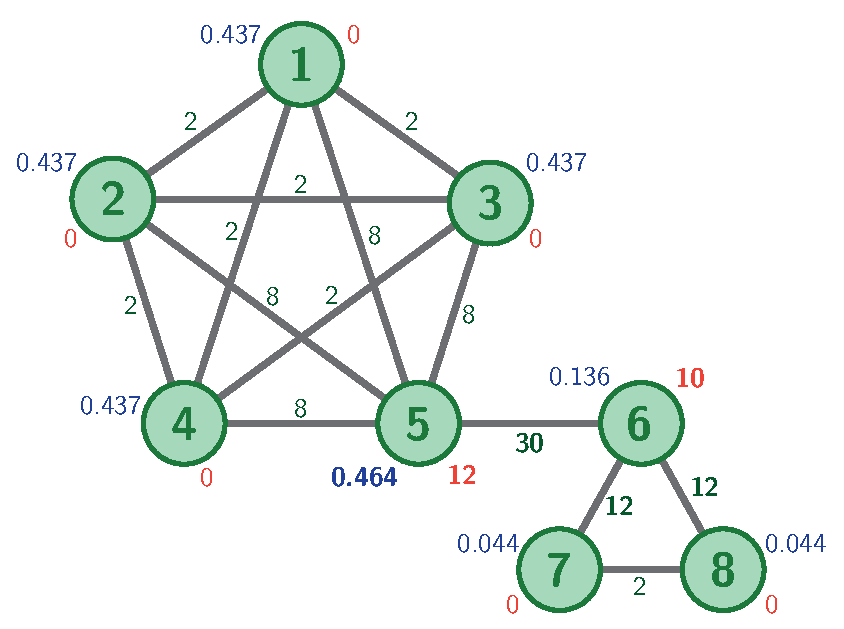
\includegraphics[width=0.48\textwidth]{cn_a2_eigbet}
    \caption{The given network with eigenvector centrality (blue) and betweenness centrality (red)}
    \label{fig:eigbet}
    \vspace{-1em}
\end{wrapfigure}
\noindent
Figure~\ref{fig:eigbet} shows the result in the graph. Eigenvector centrality of each vertex is shown by a blue decimal number next to it. As we can see, vertex number 5 has the highest eigenvector centrality means that vertex number 5 is the most \emph{central} vertex. By looking at the graph, we can intuitively understand this fact.
\newline
\noindent
\emph{Betweenness centrality} is another metric to measure how important a vertex is within the network. Different from other metric, betweenness centrality measure how important a vertex is in the information flow between other vertices. In \cite{net}, the author defines betweenness centrality $x_i$ of vertex $i$ as follow:
$$ x_i = \displaystyle \sum_{st} \frac{n_{st}^i}{g_{st}} $$
where $n^i_{st}$ is the number of geodesic paths between vertex $s$ and vertex $t$ that go through $i$, and $g_{st}$ is the total number of geodesic paths between $s$ and $t$. Besides the normal betweenness centrality, in \cite{net} the author also mentioned 2 other types of betweenness: \emph{flow betweenness} and \emph{random walk betweenness}. However, in this assignment, I will only compute the standard betweenness for the given network.

\begin{lstlisting}[language=Python, caption={Eigenvector centrality computation with SNAP.PY}]
 # Extracted from UnweightedUndirectedGraph class - File: cn_a1_p1.py
 ...
 import snap as sn
 self._graph = sn.LoadEdgeList(sn.PUNGraph, edge_list, 0, 1, ' ')
 ...
 # Compute eigenvector centrality and store to a hash table.
 def EigenvectorCentrality(self):
     # Create a hash map: Int -> Float
     NIdEigenH = sn.TIntFltH()
     sn.GetEigenVector(self._graph, NIdEigenH)
     return NIdEigenH
     \label{lst:eig}
\end{lstlisting}


\bibliography{cn_a2}

\end{document}
